
\begin{twmwindow}[\textwidth]{NgTrDat@cv-terminal:\textasciitilde}
    \powerprompt{NgTrDat}{Wed 8 Apr - 17:05}{\textasciitilde}{1}
    fastfetch -c \$HOME/.config/fastfetch/CV.jsonc

    \vspace{10pt}

    \begin{minipage}[t]{0.3\textwidth}
        \vspace{0pt}
        \centering
        \tcbox[enhanced, boxsep=0pt, left=0pt, right=0pt, top=0pt, bottom=0pt,
            arc=5pt, boxrule=1pt, colframe=winborder, clip upper, nobeforeafter]%
        {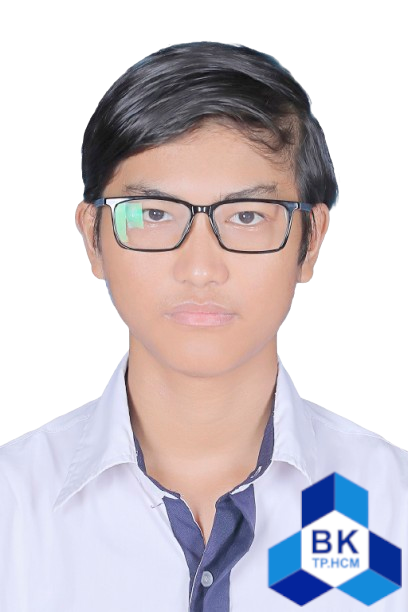
\includegraphics[height=12\baselineskip]{figure/MeFaceBK.png}}
    \end{minipage}%
    \hspace{0.03\textwidth}%
    \begin{minipage}[t]{0.65\textwidth}
        \vspace{0pt}
        \begin{Verbatim}[commandchars=\\\{\}]
\textcolor{promptblue}{NgTrDat@\textbf{cv-terminal}} 
------------------------------------------------------
\textcolor{promptgreen}{Name}       : \textbf{Nguyễn Trọng Đạt}
\textcolor{promptgreen}{Age-Gender} : \textbf{22 - Male}
\textcolor{promptgreen}{Role}       : \textbf{Computer Engineering}
\textcolor{promptgreen}{Study}      : \textbf{Ho Chi Minh University of Technology}
\textcolor{promptgreen}{Focus}      : \textbf{Robotics • AI • Drones • Embedded Systems}
\textcolor{promptgreen}{Location}   : \textbf{Ho Chi Minh City, Vietnam}
\textcolor{promptgreen}{Email}      : \href{mailto:trongdat4work@gmail.com}{\textcolor{link}{trongdat4work@gmail.com}}
\textcolor{promptgreen}{Languages}  : \textbf{C/C++, Python, Shell script}
\textcolor{promptgreen}{Tools}      : \textbf{VSCode, Git, ROS2, Gazebo}
\textcolor{promptgreen}{English}    : \textbf{TOEIC L&R \textcolor{promptgreen}{970}/990}
------------------------------------------------------
        \end{Verbatim}
    \end{minipage}

    \vspace{10pt}
    \powerprompt{NgTrDat}{Wed 8 Apr - 17:06}{\textasciitilde}{1}
    ./script/ShowMyCV.sh

\end{twmwindow}

\twmhline 

\begin{twmnotebook}[\dimexpr 0.6\textwidth-2pt\relax]{Professional\_objective.txt}[15pt][equal height group=row2]
\textbullet Computer Engineering student focused on robotics, embedded systems, and autonomous drone software. \textcolor{chillblue}{Experienced with ROS2, PX4, Gazebo, and C++ development} for real-time systems and simulation environments.\\
\textbullet Experienced in collaborative development environments using Git; proficient at reading, understanding, and contributing safely to shared codebases.\\
\textbullet Seeking a part-time engineering role, potentially transitioning to full-time after graduation.
\end{twmnotebook}%
\twmgap
\begin{twmimage}[\dimexpr 0.4\textwidth-2pt\relax]{Drone\_Simulation\_Preview.png}[equal height group=row2]
    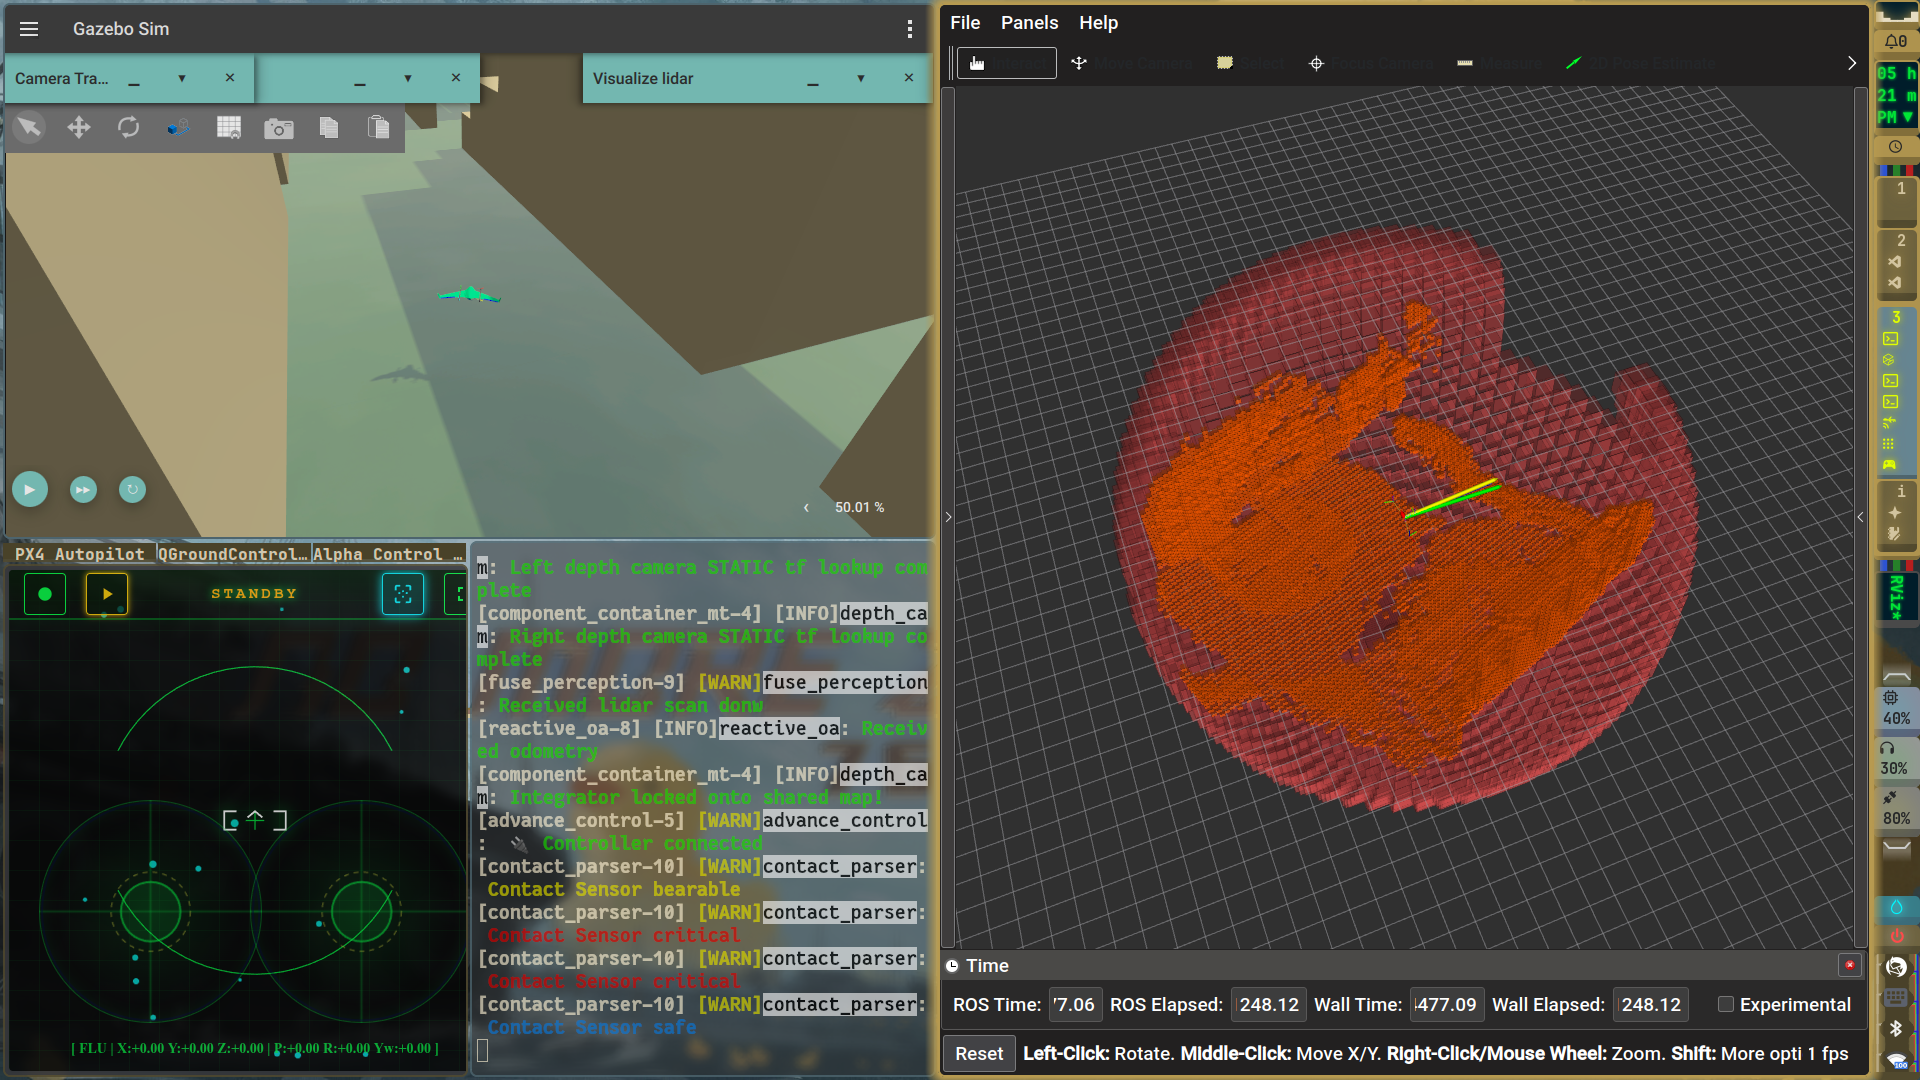
\includegraphics[width=\linewidth]{figure/DemoDrone.png}
\end{twmimage}

\twmhline

\begin{twmnotebook}[\dimexpr \textwidth-2pt\relax]{Education.log}[0pt]
    \cvrow{{[Study]}}{Ho Chi Minh University of Technology (BKU)}
    \cvrow{{[Major]}}{Bachelor of Engineering in Computer Engineering (Expected graduation 2027)}
    \cvrow{{[GPA]}}{2.9/4.0}
    \cvrow{{[Core Coursework]}}{
        \textbullet \quad Embedded System \qquad \textbullet \quad Operating System \qquad \textbullet \quad Machine Learning\newline
        \textbullet \quad Microprocessors-Microcontrollers \newline
        \textbullet \quad IoT-Oriented Logic Design Project \newline
        \textbullet \quad AI-Oriented Multidisciplinary Project
    }
    \cvrow{{[Passion Project]}}{\textcolor{chillblue}{Developed a ROS2 and PX4 drone simulation pipeline in Gazebo to train AI models for VTOL acrobatic flight.}}
\end{twmnotebook}

\twmhline
\begin{twmimage}[\dimexpr 0.3\textwidth-2pt\relax]{LIDAR\_depth\_scan.png}[equal height group=row4, valign=center, halign=center]
    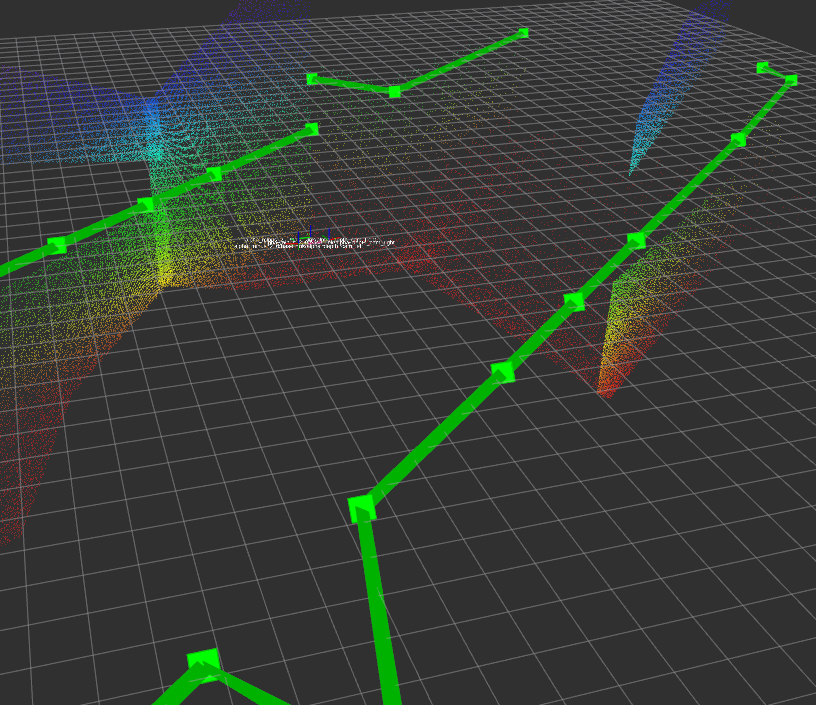
\includegraphics[width=\textwidth]{figure/depth_map.png}
\end{twmimage}%
\twmgap
\begin{twmide}[\dimexpr 0.7\textwidth-2pt\relax]{Skills.md}[equal height group=row4, colback=idebg, coltext=idefgchill]
    \begin{Verbatim}[commandchars=\\\{\}, numbers=left, numbersep=12pt, formatcom=\color{idefg}]
\textcolor{chillgreen}{\textbf{Programming:}}
  \textcolor{chillgreen}{\textbullet} Most proficient with \textcolor{promptblue}{C++}, \textcolor{promptblue}{Python} and \textcolor{promptblue}{Rust}
  \textcolor{chillgreen}{\textbullet} Familiar with Java, Go, Zig
\textcolor{chillgreen}{Robotics \& Middleware ecosystem:}
  \textcolor{chillgreen}{\textbullet} \textcolor{promptblue}{ROS2 (Jazzy)} \quad \textcolor{chillgreen}{\textbullet} \textcolor{promptblue}{Gazebo Harmonic}
  \textcolor{chillgreen}{\textbullet} PX4 Autopilot \quad \textcolor{chillgreen}{\textbullet} MicroXRCE-DDS
\textcolor{chillgreen}{AI, Machine Learning and Data Engineering:}
  \textcolor{chillgreen}{\textbullet} Latent Diffusion Learning \quad \textcolor{chillgreen}{\textbullet} Robotic data processing
  \textcolor{chillgreen}{\textbullet} Reinforcement Learning \quad \textcolor{chillgreen}{\textbullet} AI Edge Computing
\textcolor{chillgreen}{Development tools:} \textcolor{chillgreen}{\textbullet} VScode \quad \textcolor{chillgreen}{\textbullet} \textcolor{promptblue}{Git} \quad \textcolor{chillgreen}{\textbullet} \textcolor{promptblue}{Linux OS}
    \end{Verbatim}
\end{twmide}

\twmhline

\begin{twmnotebook}[\dimexpr 0.5\textwidth-2pt\relax]{Contacts.txt}[0pt][equal height group=row5]
{\Large } \quad Phone : (+84) 399922395\\
{\Large } \quad Email : \href{mailto:trongdat4work@gmail.com}{\textcolor{link}{trongdat4work@gmail.com}}\\
{\Large } \quad Github: \href{https://github.com/LemonKronos}{\textcolor{link}{github.com/LemonKronos}}\\
{\Large } \quad LinkIn: \href{https://www.linkedin.com/in/trong-dat}{\textcolor{link}{www.linkedin.com/in/trong-dat}}\\
\textcolor{gray}{* All source code below is available on GitHub}
\end{twmnotebook}%
\twmgap%
\begin{twmnotebook}[\dimexpr 0.5\textwidth-2pt\relax]{About\_me.txt}[0pt][equal height group=row5]
\textbullet \quad I am a \textcolor{chillblue}{Drone enthusiast}\\
\textbullet \quad My goal is to become a Robotics Engineer\\
\textbullet \quad Open-source mindset, member of Linux community\\
\textbullet \quad Strong technical communicator, ready to collaborate in international teams\\
\end{twmnotebook}